\documentclass{beamer}

\usepackage{amsmath, amssymb}
\usepackage{graphicx}
\usepackage{url}
\usepackage{xspace}
\usepackage{pifont}
\usepackage{minted}
\usepackage{verbatim}
\usepackage{wasysym}
\usepackage[notocbib]{apacite}
\usepackage{bm}

\usetheme{AnnArbor}
\usefonttheme[onlymath]{serif}

\newcommand\blfootnote[1]{%
  \begingroup
  \renewcommand\thefootnote{}\footnote{#1}%
  \addtocounter{footnote}{-1}%
  \endgroup
}

\DeclareMathOperator{\Tr}{Tr}
\DeclareMathOperator*{\argmin}{arg\,min}

\title[PnS2018]{\textbf{PnS 2018} \\
\textbf{\normalsize Deep Learing with Raspberry Pi}\\
\normalsize Session 3}
\author{PnS 2018 Team}
\institute[INI-UZH/ETHz]{Institute of Neuroinformatics \\
University of Z\"urich and ETH Z\"urich}

\date{}

\begin{document}

\titlepage

\begin{frame}
\frametitle{Outline}

\tableofcontents
\end{frame}

\section{Multi-Layer Perceptron}

\begin{frame}
  \frametitle{Artifical Neuron: Overview}
  \begin{columns}
  \column{0.5\textwidth}
  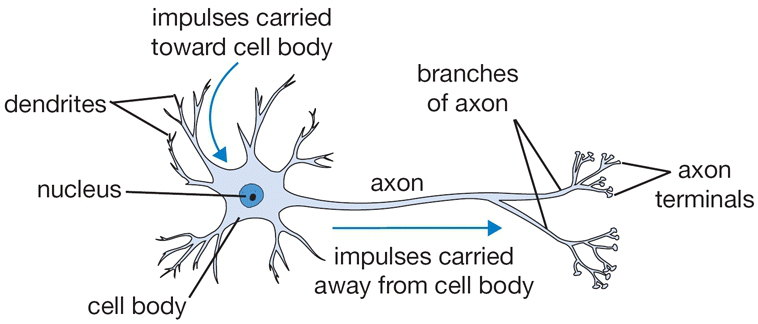
\includegraphics[width=\textwidth]{neuron.png}
  \column{0.5\textwidth}
  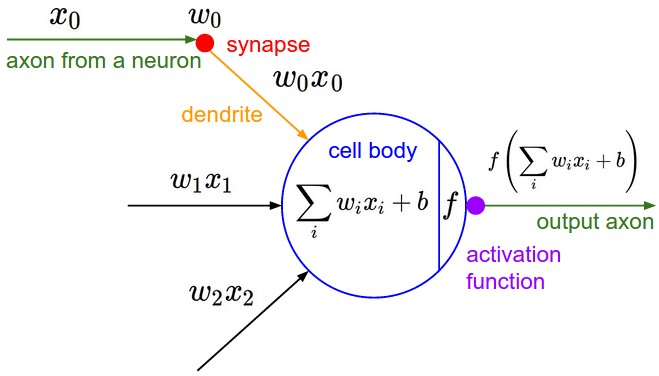
\includegraphics[width=\textwidth]{neuron_model.jpeg}
  \end{columns}
  \begin{itemize}
  \item A basic computational model of the biological model
  \item Single neuron as linear/logistic regression
  \end{itemize}
  \blfootnote{http://cs231n.github.io/neural-networks-1/}
\end{frame}

\begin{frame}
  \frametitle{Multi-Layer Perceptron}
  \begin{columns}
  \column{0.45\textwidth}
  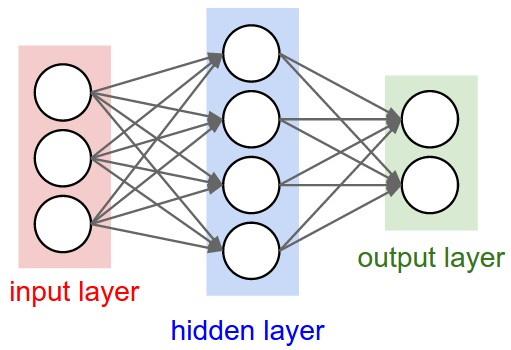
\includegraphics[height=1.3in]{neural_net.jpeg}
  \column{0.55\textwidth}
  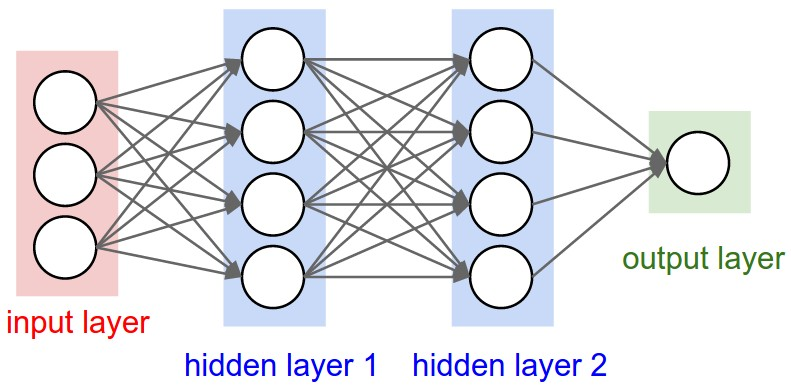
\includegraphics[height=1.3in]{neural_net2.jpeg}
  \end{columns}
  \begin{itemize}
  \item Neurons in an acyclic feed-forward graph
  \item Fully connected layers
  \item Each fully connected layer computation is a matrix multiplication,
    matrix addition and an activation function
  \end{itemize}
  \blfootnote{http://cs231n.github.io/neural-networks-1/}
\end{frame}

\begin{frame}
  \frametitle{What can an MLP learn?}
  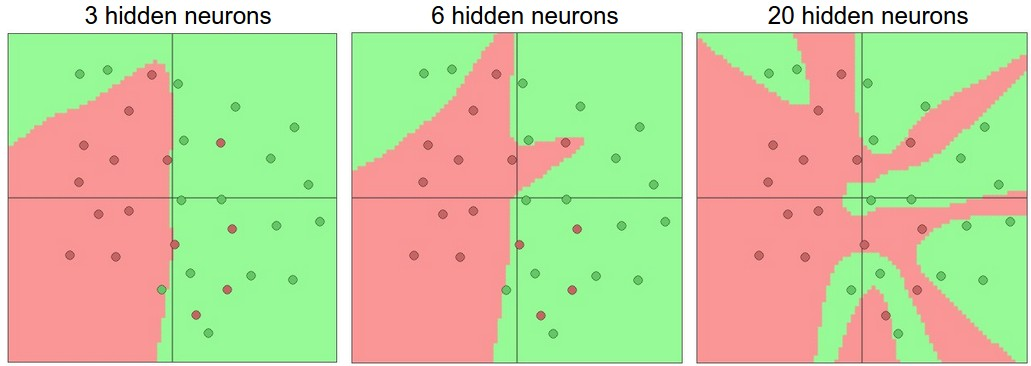
\includegraphics[width=\textwidth]{layer_sizes.jpeg}
  \begin{itemize}
  \item Neural Networks with at least one hidden layer are universal
    approximators\footnote{Approximation by superpositions of a sigmoidal function, by Cybenko G.}
  \item More neurons are expected to approximate better
  \end{itemize}
  \blfootnote{http://cs231n.github.io/neural-networks-1/}
\end{frame}

\section{Regularization}

\begin{frame}
  \frametitle{Regularization}
  \begin{itemize}
  \item Overfitting more probable with larger models
  \item Could be prevented by using a regularization term in the loss function
  \end{itemize}
\end{frame}

\begin{frame}
  \frametitle{Regularization}
  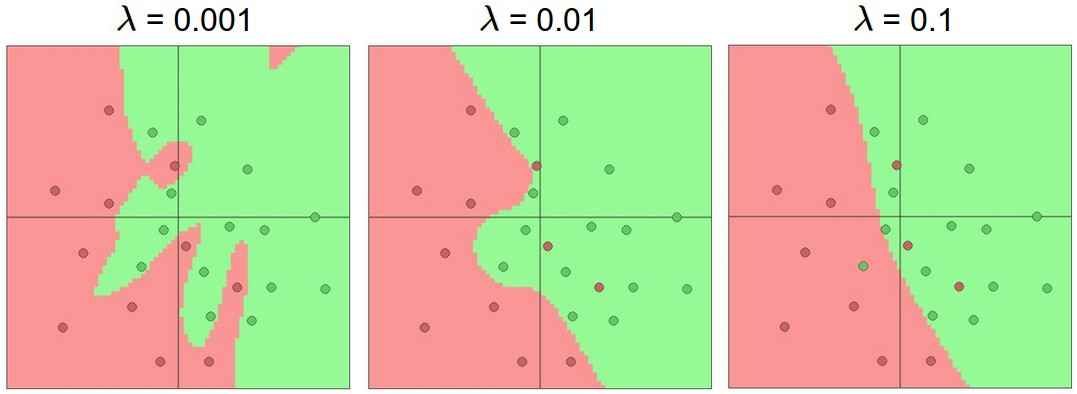
\includegraphics[width=\textwidth]{reg_strengths.jpeg}
  \begin{itemize}
  \item Use bigger networks but take measures to prevent overfitting
  \end{itemize}
  \blfootnote{http://cs231n.github.io/neural-networks-1/}
\end{frame}

\section{Convolutional Neural Networks}

\begin{frame}
  \frametitle{Working with images}
  \begin{itemize}
  \item MLPs do not work well with images
  \item Hierarchy of local spatial features
  \item Extract these local spatial features through filters
  \end{itemize}
\end{frame}


\end{document}
%%% Local Variables:
%%% mode: latex
%%% TeX-master: t
%%% End:
